\section{隐通道构建}
\label{chap:hash:designation}

本节对该时间隐通道构建方法进行总体描述,首先介绍时间隐通道的设计架构,然后展开介绍调制流程及数据转换过程,最后介绍解调过程及数据转换过程。

\subsection{设计架构}
\label{chap:hash:designation:model}

\insertFigure{
	\begin{figure}[htbp]
		\centering
        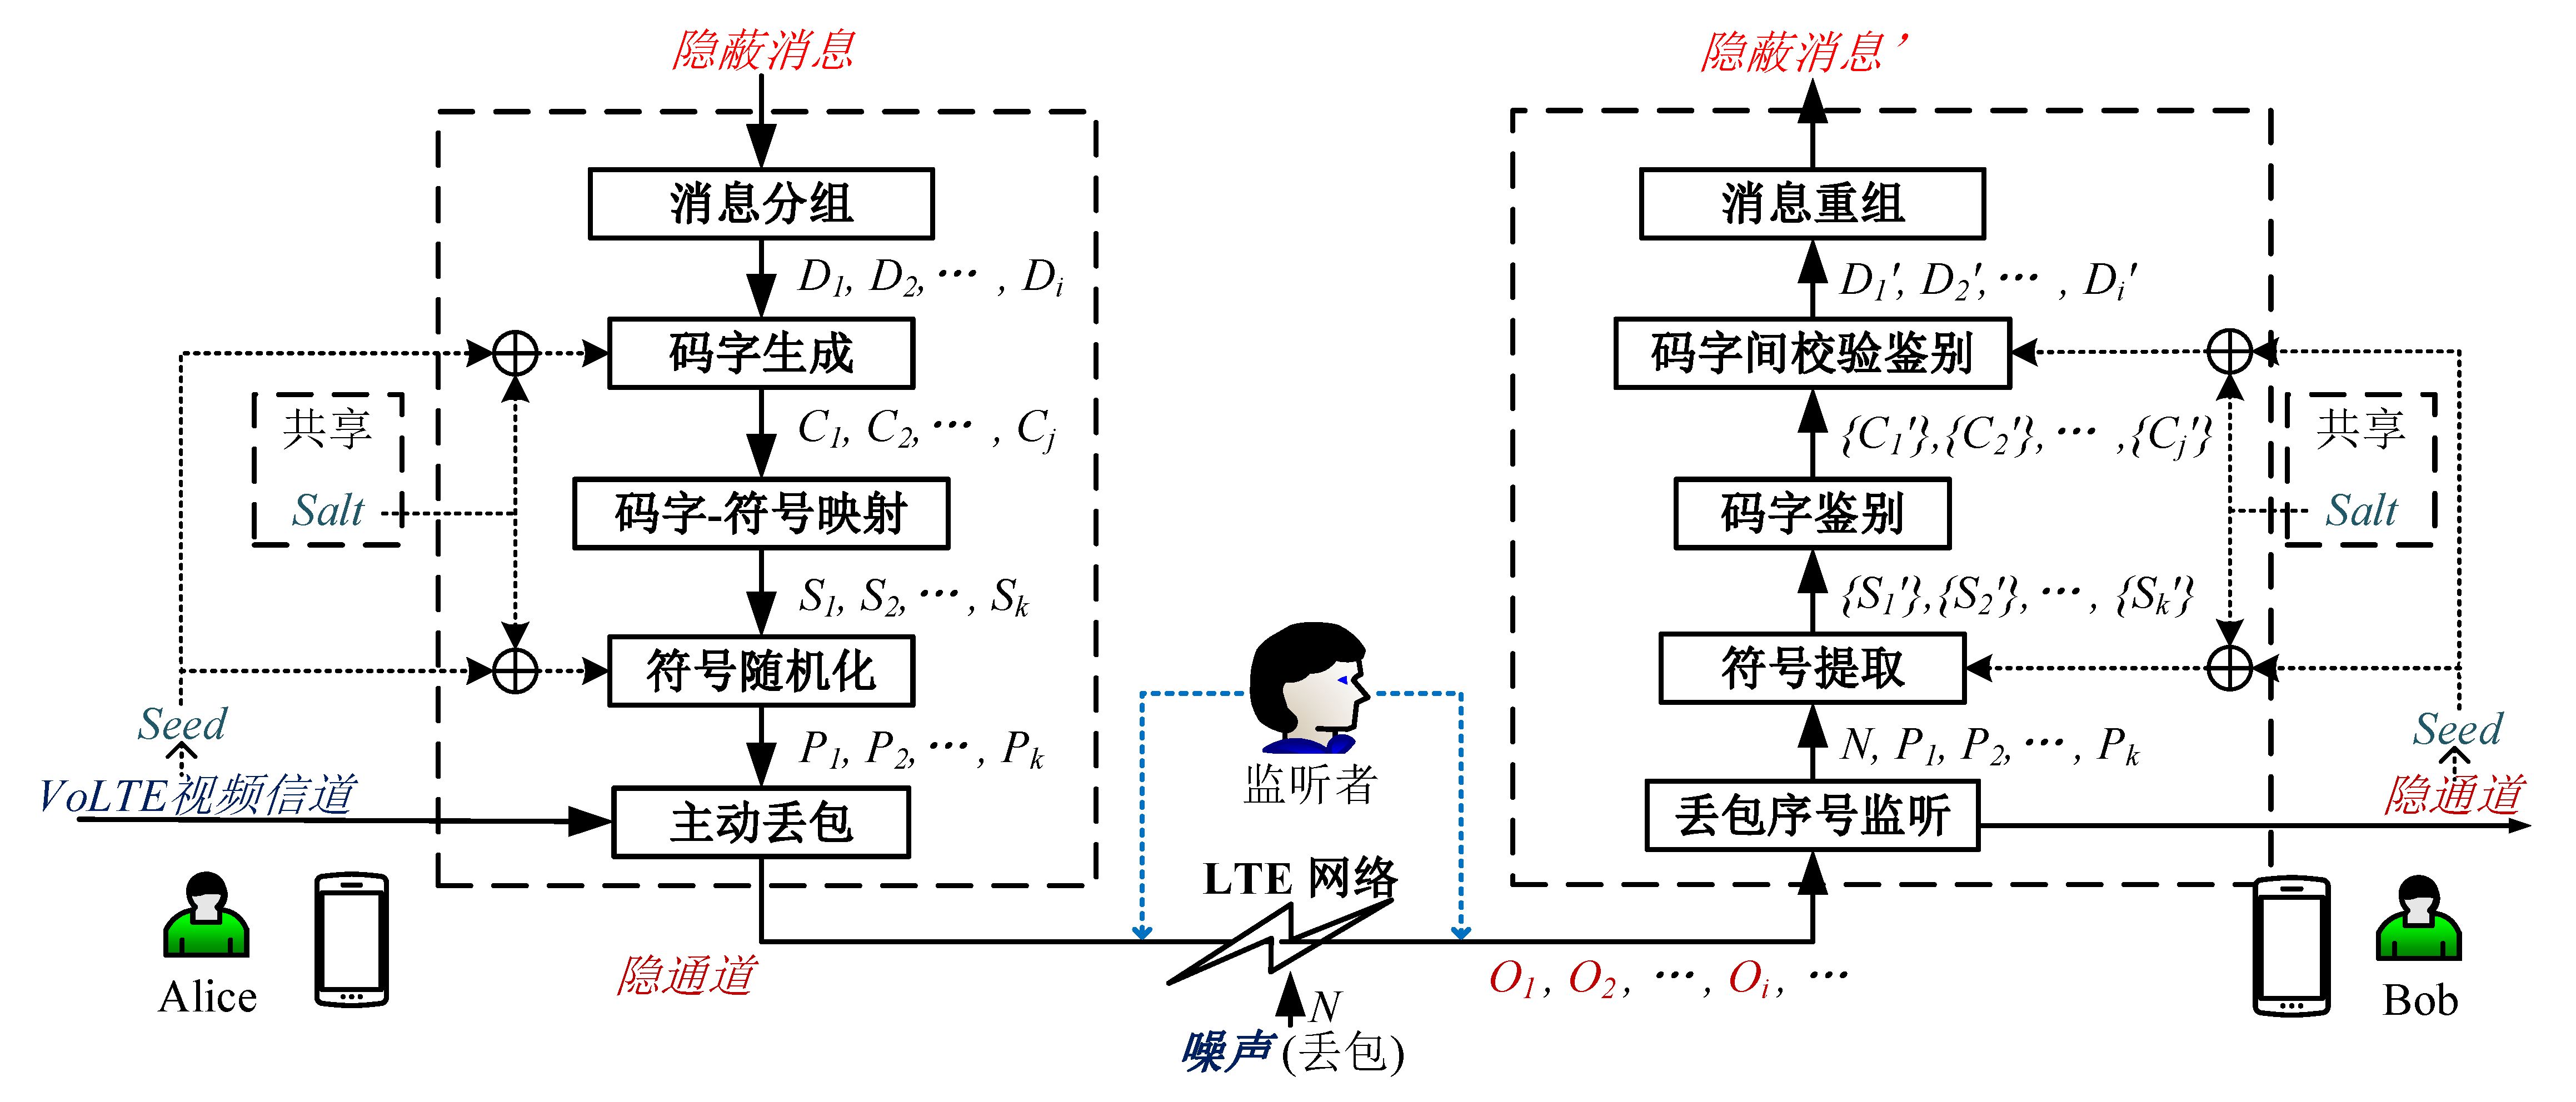
\includegraphics[width=0.99\textwidth]{chapters/chapter5/figures/system-model.pdf}
        \caption{基于多重校验纠错的时间隐通道设计架构图}
        \label{fig:5:system-model}
    \end{figure}
}

该时间隐通道构建方法的设计架构如图\nref{fig:5:system-model},对于发送方Bob和接收方Alice,需要躲避监听者传输隐蔽消息。为确保消息保密性,双方约定共享变量$Salt$,用于增加传输过程的随机性。发送方首先将隐蔽消息分组,得到消息块$D_{i}$。接下来,码字生成过程根据私有$Salt$及RTP中的随机字段$Seed$,计算码字间校验信息及码字自校验信息,形成码字$C_{j}$。然后参照映射矩阵,将码字映射为符号$S_{k}$,也就是相对丢包位置。符号随机化过程为每一组的符号添加随机偏移量,并转换为要丢弃的数据包序号$P_{k}$。

宿主信道即VoLTE视频信道,主动丢包过程将特定序号的数据包丢弃后,时间隐通道构建完毕。经LTE网络传输后,接收方执行隐通道解调操作。监听者位于LTE网络,能够监听和控制所有数据包。

解调过程中,接收方监听数据包传输情况,得到丢失数据包序号$P_{k}$。参照映射矩阵及校验规则,符号提取过程将丢包序号转换为候选符号集合$\{S_{k}'\}$。符号提取过程同时消除每组符号的随机偏移量,依据双方共享的私有$Salt$及RTP导出的$Seed$。码字鉴别过程将符号转换为候选码字,同时验证码字中基于CRC的码字自校验信息,输出每组的候选码字集合$\{C_{j}'\}$。码字间校验鉴别阶段,对码字间校验关系进行验证,筛选出概率最大的组合,并导出为消息块$D_{i}'$。最终,将消息块进行重新组合,接收方得到隐蔽消息,时间隐通道传输完毕。

\subsection{调制流程}
\label{chap:hash:designation:modulation}

\insertFigure{
    \begin{figure}[htb]
        \centering
        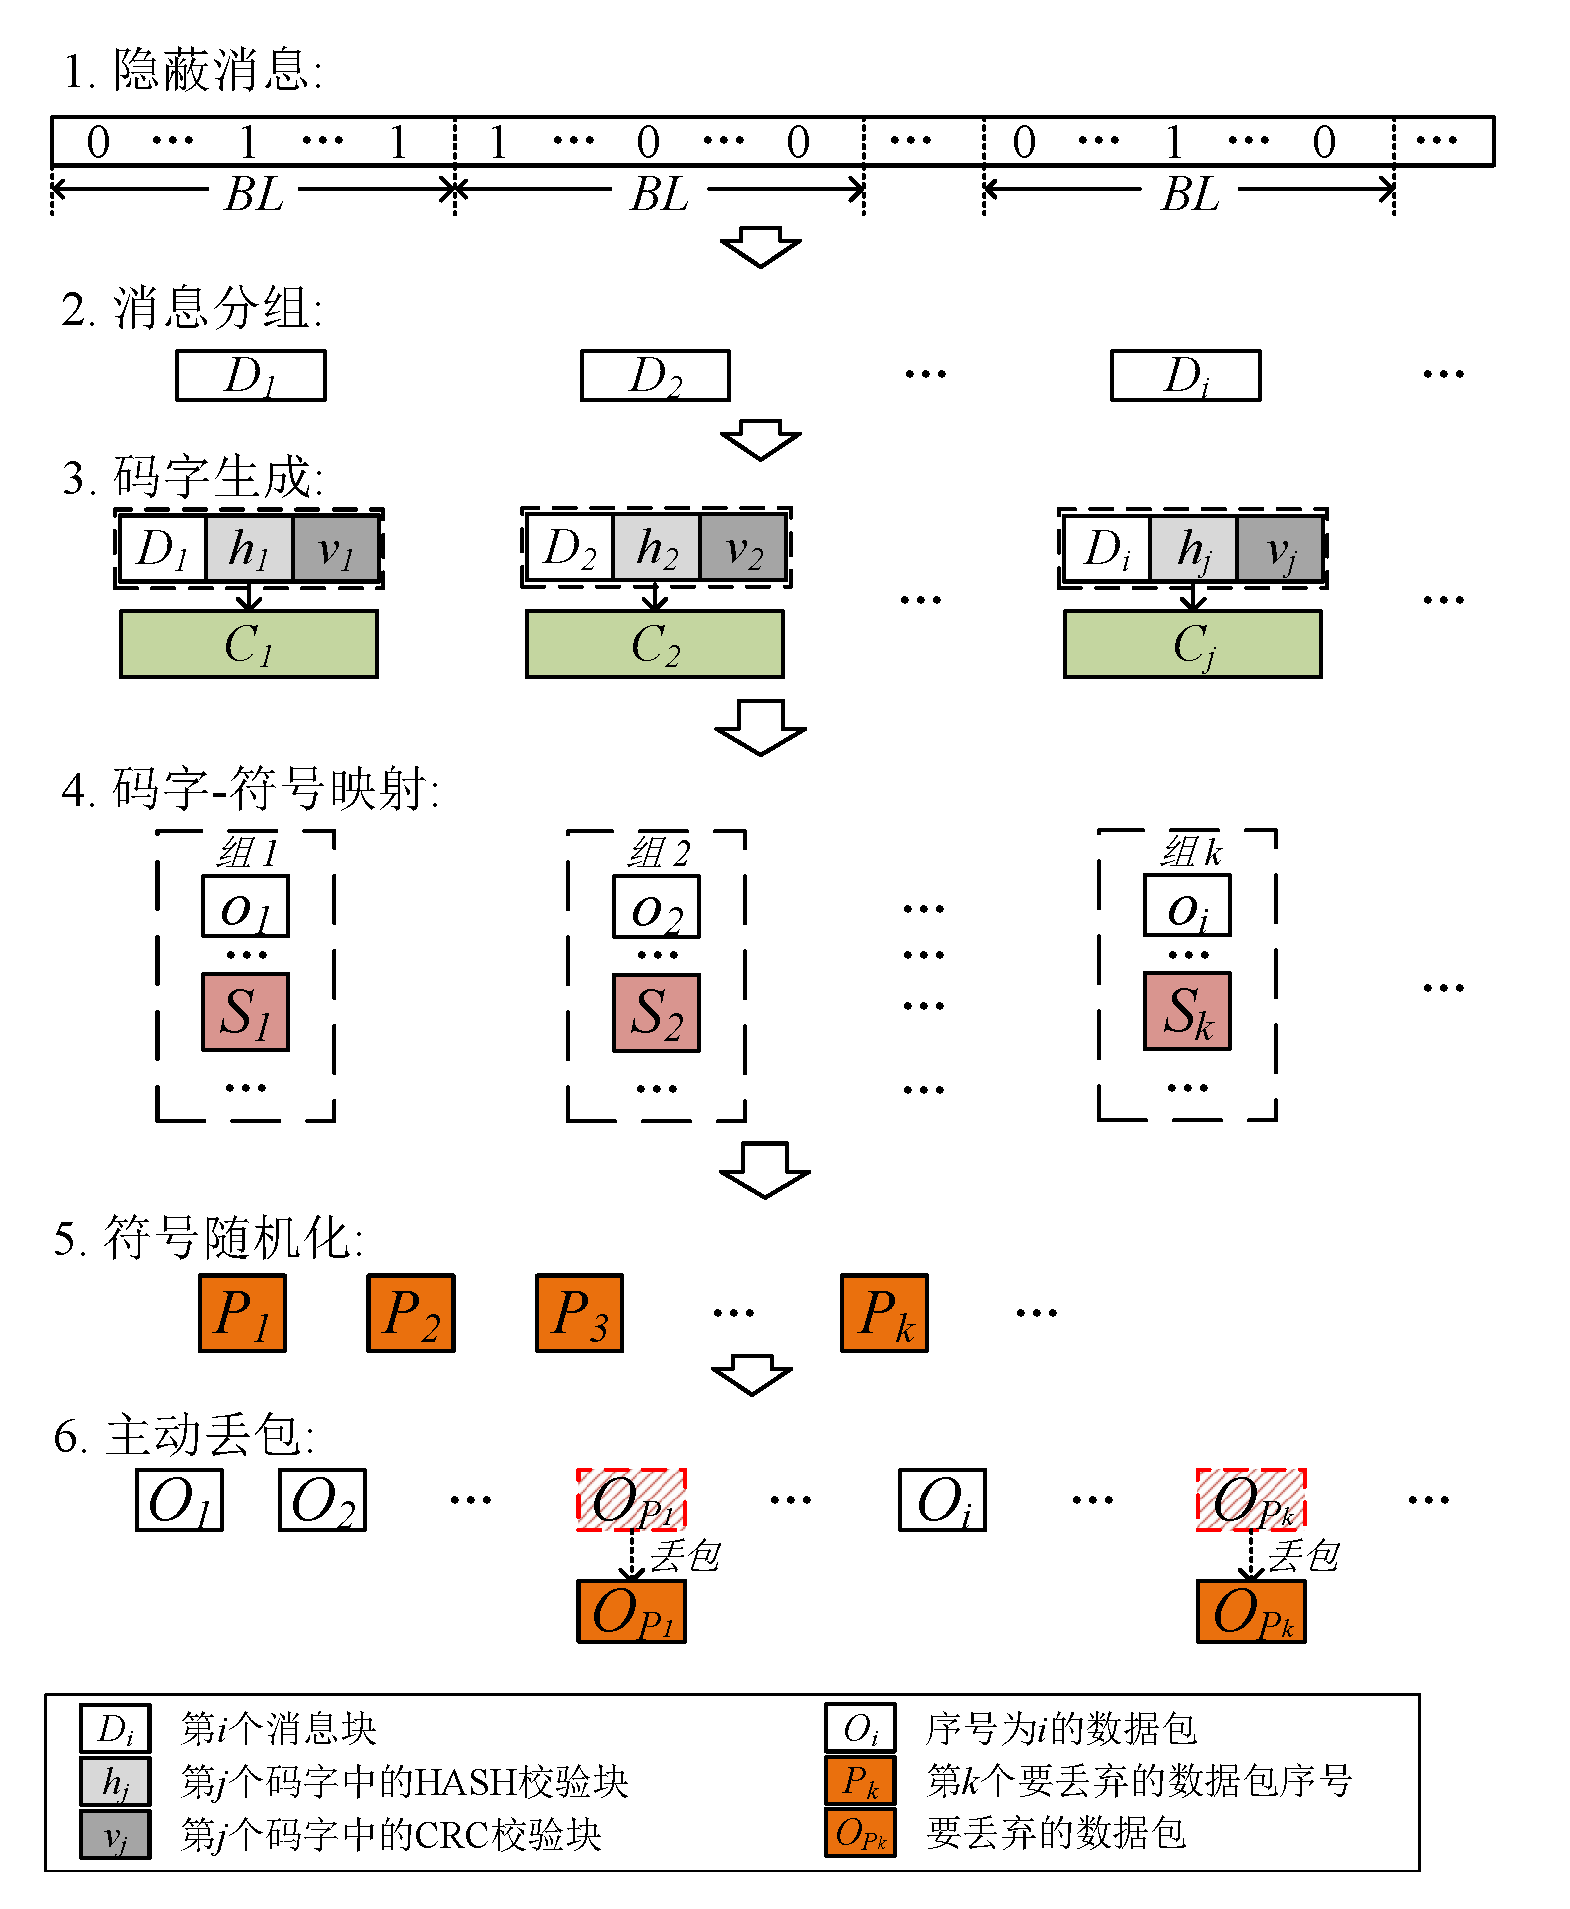
\includegraphics[width=0.75\textwidth]{chapters/chapter5/figures/modulation-flow.pdf}
        \caption{基于多重校验纠错的时间隐通道调制流程}
        \label{fig:5:modulation-flow}
    \end{figure}
}

如图\nref{fig:5:modulation-flow},调制过程中的数据流变化主要分为五个部分,与时间隐通道架构中的流程基本一致。首先对隐蔽消息进行分组,每个数据块的长度为$BL$,得到等长数据块$\{D_{1},\ D_{2},\ \cdots ,\ D_{i}\}$。接下来,在每个数据块的基础上计算基于HASH的码字间校验,并由摘要结果中提取{$L_{HASH}$\ bits},作为$h_{j}$,拼接到$D_{i}$尾部。对于每一个$\{D_{i}\ //\ h_{j}\}$组合,计算其CRC散列值,并由结果中提取{$L_{CRC}$\ bits}作为$v_{j}$。最后将$\{D_{i},\ h_{j},\ v_{j}\}$按序组合,得到码字$C_{j}$。因此,$L_{Codeword}$与$BL$、$L_{HASH}$及$L_{CRC}$的关系,如公式(\nref{equ:5:codeword-length})。
\insertEquation{
    \begin{equation}
    \label{equ:5:codeword-length}
		L_{Codeword}\ =\ BL\ +\ L_{HASH}\ +\ L_{CRC}
    \end{equation}
}
码字-符号映射过程,将二进制的码字$C_{j}$,转换为每组中的相对偏移量$S_{k}$。在映射过程中,添加异或校验符号,因此$S_{k}$的数量多于$C_{j}$的数量。接下来,进行符号随机化过程,基于传入的随机数种子,迭代伪随机数发生器,为每一组符号添加随机偏移量。伪随机数发生器在种子一致的情况下,具有相同的随机数序列,因此接收方能够完全还原。通过结合用户自定义的随机数种子,及RTP中的SSRC随机字段,确保每次通话的丢包位置不同,抵御重放攻击、增强保密性。最后,将符号转换为数据包序号$P_{k}$,由主动丢包过程丢弃,调制过程结束。

\subsection{解调流程}
\label{chap:hash:designation:demodulation}

\insertFigure{
    \begin{figure}[htb]
        \centering
        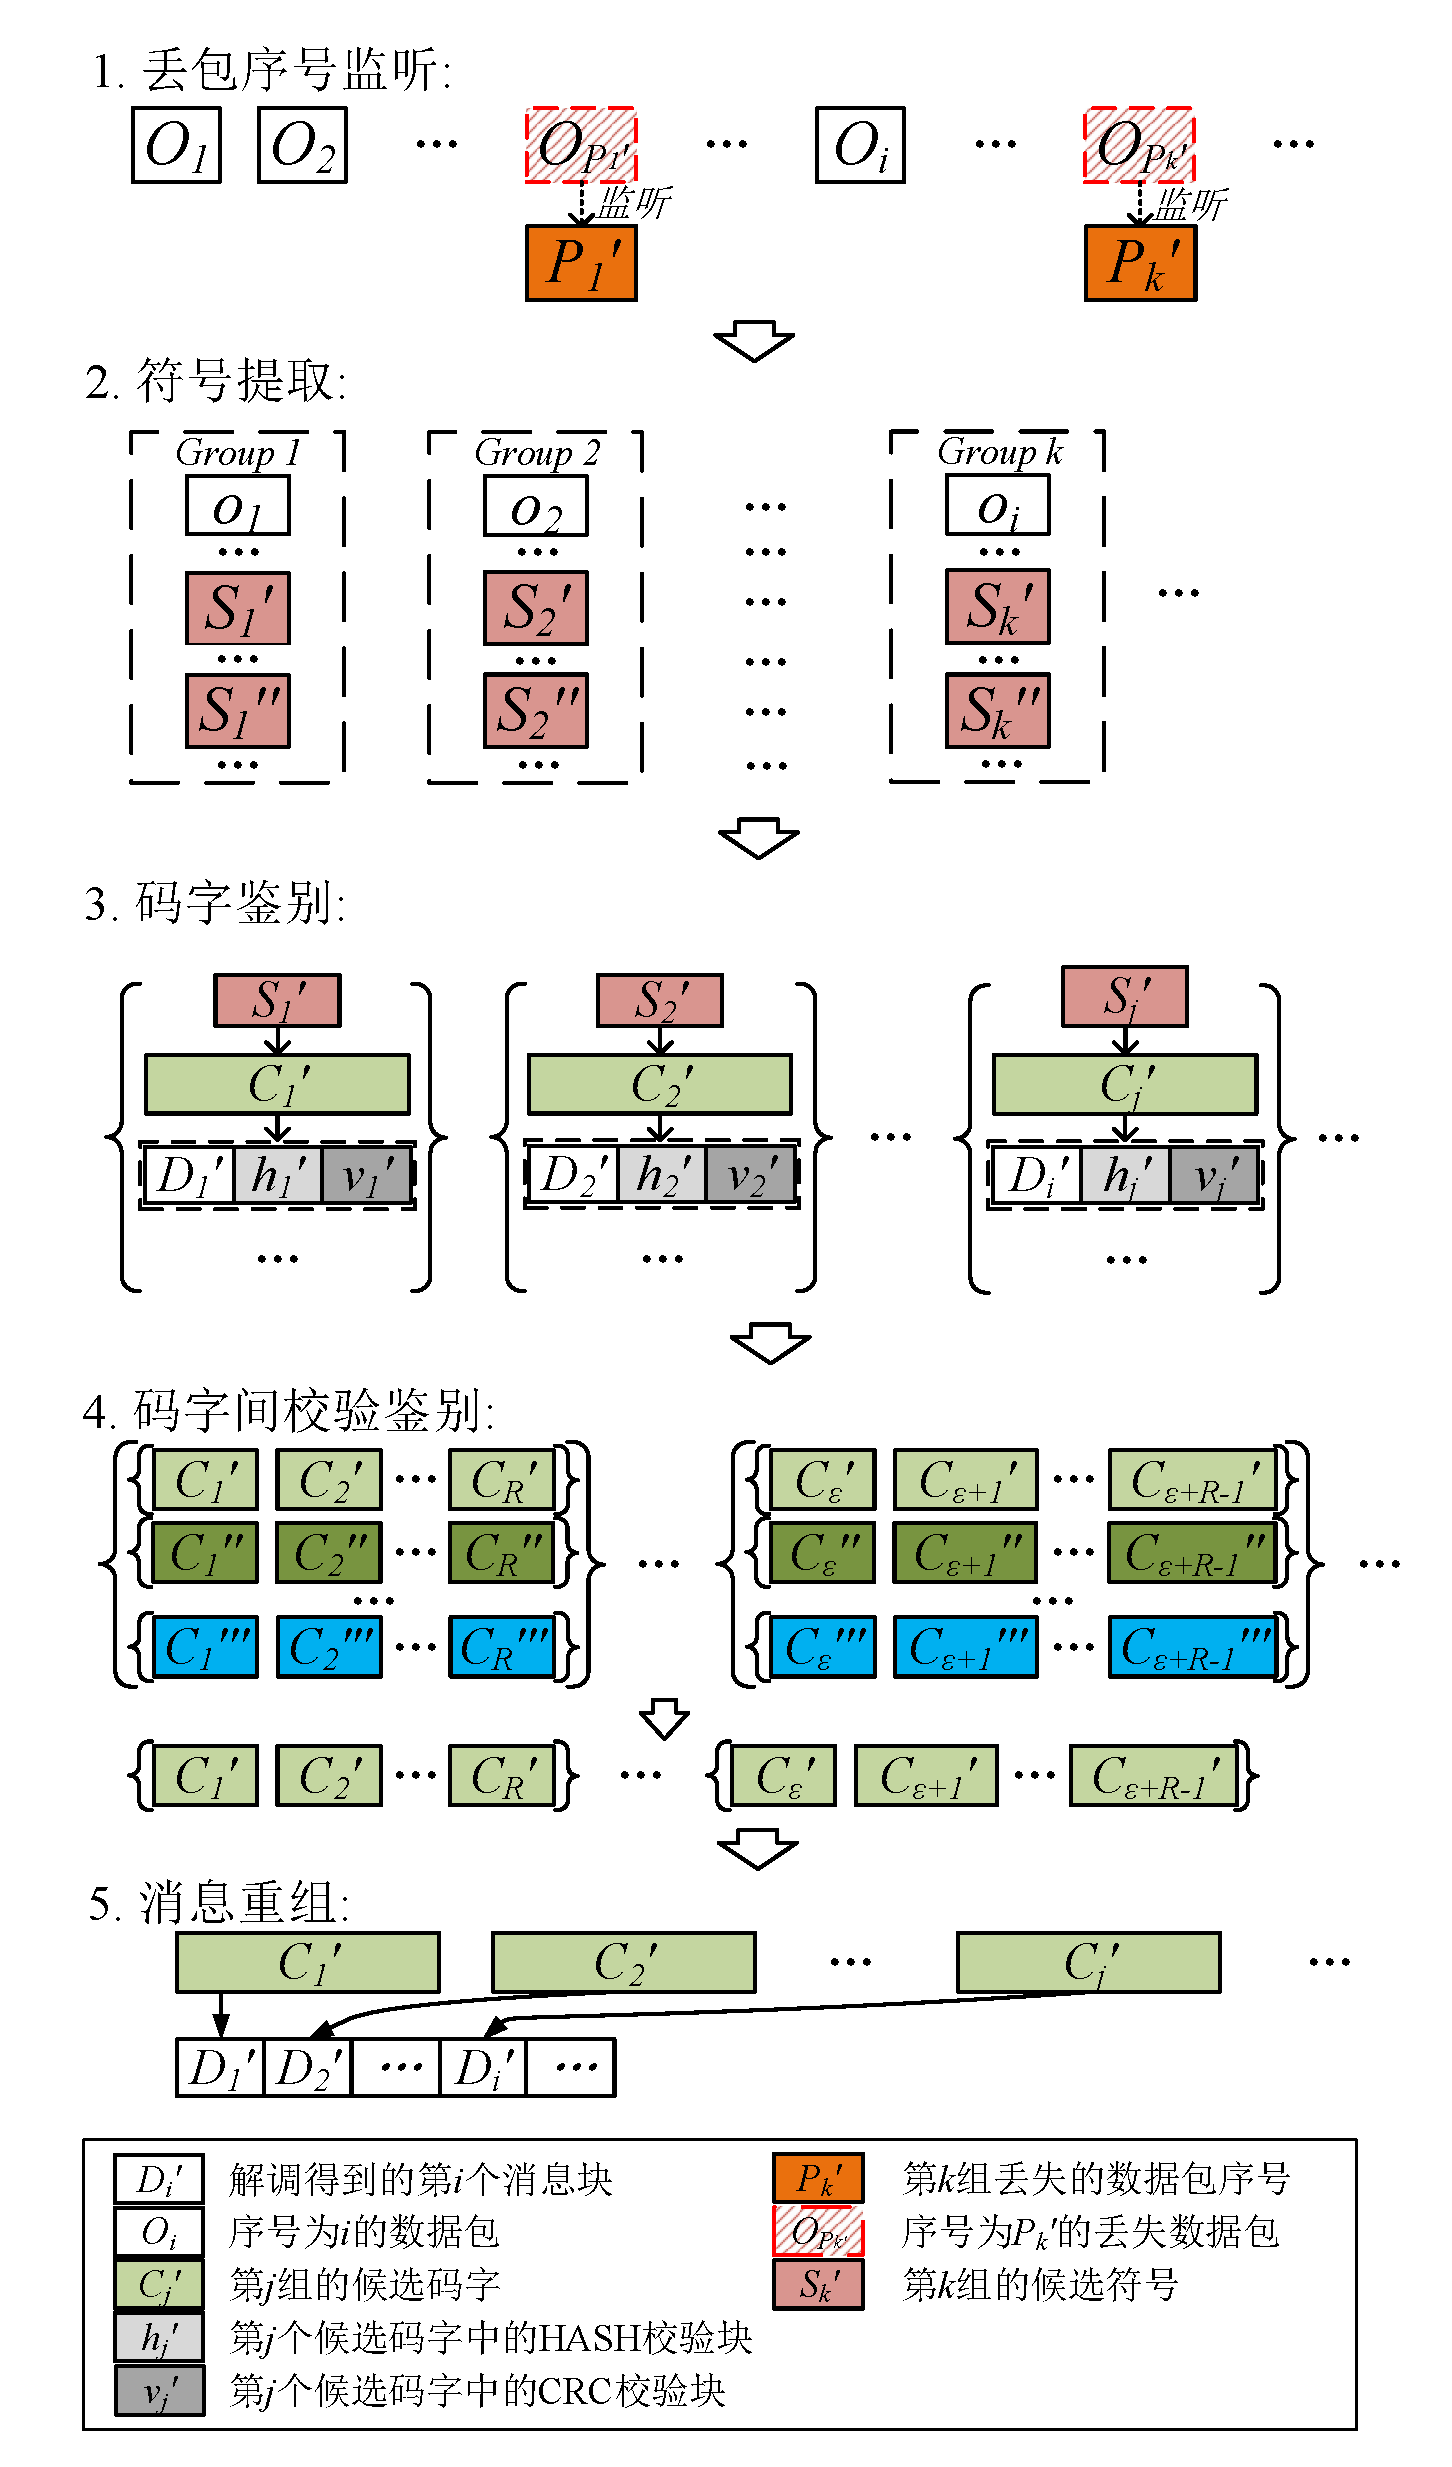
\includegraphics[width=0.7\textwidth]{chapters/chapter5/figures/demodulation-flow.pdf}
        \caption{基于多重校验纠错的时间隐通道解调流程}
        \label{fig:5:demodulation-flow}
    \end{figure}
}

如图\nref{fig:5:demodulation-flow},解调过程的数据流程主要包括五个部分,与图\nref{fig:5:system-model}的解调过程对应。丢包序号监听分析当前接收到的数据包序号,根据序号的空缺情况,得到丢失数据包序号$P_{k}'$。符号提取过程将序号转变为每组的符号,由于网络噪声不可避免,因此每组的候选符号为集合$\{S_{k}',\ S_{k}'',\ \cdots \}$。

对于候选符号$\{S_{k}',\ S_{k}'',\ \cdots \}$,根据随机数种子迭代伪随机数生成器,消除符号中的随机偏移量。通过验证异或校验关系,鉴别出符合规则的数据符号。

码字鉴别过程,首先对码字中包含的$v_{j}$部分进行验证,得到符合规则的候选码字。接下来对码字中包含的$h_{j}$部分进行验证,按照码字间校验的模式,遍历所有的码字组合,校验失败则意味着组合无效。最终,得到一组具有最大概率的码字组合$\{C_{1}',\ C_{2}',\ \cdots,\ C_{j}'\}$。最后的消息重组过程,将码字中的数据块$D_{i}$按序组合得到隐蔽消息。

该时间隐通道构建方法自带传输同步能力,无需同步时钟也可保证消息顺序。通过结合码字间校验、码字自校验、符号间校验及映射矩阵,逐层降低噪声强度,提高了时间隐通道的鲁棒性。